\clearpage
\section{关闭通讯窗口时误触游戏操作}

在独立游戏窗口中按 T 打开「队友通讯」，点右上角的叉号，窗口正常关闭。旧版里，同一次点击也能被角色脚本读到。维修站的装备脚本用鼠标左键使用当前装备，因此关窗口也可能触发一次使用。我们在步行测试场景中加了一个 C\# 脚本，只记下鼠标左键何时按下、何时松开。这样可以直接看出点击去了哪里。

\begin{center}
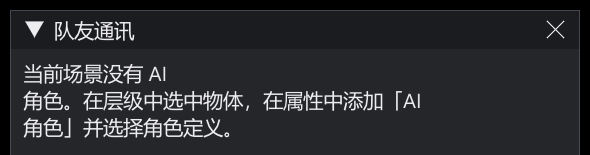
\includegraphics[width=.79\linewidth]{../../../output/validation/watt-station/hud/input/before/communications.png}\\
{\small 实际游戏窗口局部。测试点击右上角的叉号，又分别从面板内和面板外开始拖动。}
\end{center}

从 \path{RedflagForge/src/VulkanForgeLayer.cpp} 的 \texttt{DrawViewport} 查起，场景图已经用 \texttt{IsItemHovered} 判断鼠标是否指在游戏画面上，再让 \texttt{ImGuiLayer::BlockEvents} 把工具窗口的事件留给界面。C\# 游戏脚本却从另一个入口读取鼠标。在 \path{Redflag/src/Redflag/Scripting/ScriptGlue.cpp} 中，旧版的 \texttt{Input\_IsMouseButtonDown} 只有下一行。

\begin{Code}
return Input::IsMouseButtonPressed(button); // 直接读取 GLFW 的按键状态
\end{Code}

GLFW 返回的是鼠标左键目前有没有按下。ImGui 已经处理了关闭按钮，鼠标仍可能处于按下状态。修复后，游戏读取按下时的归属。若从游戏图里开始拖动，手指没有松开前，角色会一直读到按住。若从工具面板里开始拖动，即使光标移回游戏，角色也不会中途使用装备。

\loc{Redflag/src/Redflag/ImGui/ImGuiLayer.cpp}
\begin{Code}
if (ImGui::IsMouseClicked(button))
    (*m_GameMouseButtons)[button] = !block; // 按下时决定这次点击交给谁
if (!ImGui::IsMouseDown(button))
    (*m_GameMouseButtons)[button] = false; // 松开后清除这一键
\end{Code}

复测时还发现了测试工具自身的问题。在 Windows 的隔离桌面投递鼠标消息，按键状态能进入 GLFW，但按下当帧取到的指针位置可能回到 $(0,0)$。此时仅凭浮窗消失，不能确定点中了关闭按钮。正式试玩记录器把客户区坐标和按下事件一并送进 ImGui，再由实际窗口判断点击位置。全屏游戏画面保持在工具窗口下面，点回游戏也不会把通讯窗口盖住。

从仓库根目录运行 \texttt{python tests/check\_game\_mouse.py}。正式游戏窗口中，首次点击得到一对按下和松开，点通讯窗口叉号后游戏记录没有增加。从游戏向面板拖动可一直按住，从面板向游戏拖动则没有游戏输入。松开再点击游戏，脚本正常得到下一对记录。窗口局部图、逐步输入与接管回执保存在 \path{output/validation/watt-station/hud/input/}。
